\chapter{Kinetika Kimia: Hukum Laju}\label{ch:b1:rate-laws}

Susu tahan seminggu di dalam lemari es dan hanya sehari di atas meja pada
musim panas. Kemasan sebuah obat bertuliskan ``simpan di bawah
\qty{25}{\celsius}'' dan mencantumkan tanggal kedaluwarsa dua atau tiga
tahun ke depan, yang tidak sempat diamati langsung oleh pabriknya.
Tetapan kesetimbangan menyatakan di mana sebuah reaksi berakhir; tetapan
itu tidak menyatakan apa pun tentang berapa lama waktu yang diperlukan
untuk sampai ke sana. Itulah ranah kinetika kimia. Bab ini mendefinisikan
laju sebuah reaksi, hukum-hukum laju yang menyatakannya dengan
konsentrasi, bentuk-bentuk terintegrasi yang meramalkan konsentrasi pada
setiap saat, metode-metode eksperimen yang menentukan sebuah \omterm{def:b1:rate-laws:order}{hukum laju},
dan \omterm{thm:b1:rate-laws:arrhenius}{hukum Arrhenius} yang memerikan pengaruh suhu --- alat yang dipakai
untuk meramalkan masa simpan sebuah obat dalam beberapa minggu percobaan.

\begin{recall}
Buku 1 (kelas 12) memperkenalkan laju kemunculan dan \omterm{def:b1:rate-laws:rate}{laju penghilangan}
sebuah spesies, faktor-faktor kinetik (konsentrasi, suhu, katalis), dan
\omterm{def:b1:rate-laws:half-life}{waktu paruh} reaksi orde satu. Kemajuan $\xi$ sebuah reaksi didefinisikan
pada \cref{def:b1:extent-q-and-k:extent}.
\end{recall}

\begin{omfigure}
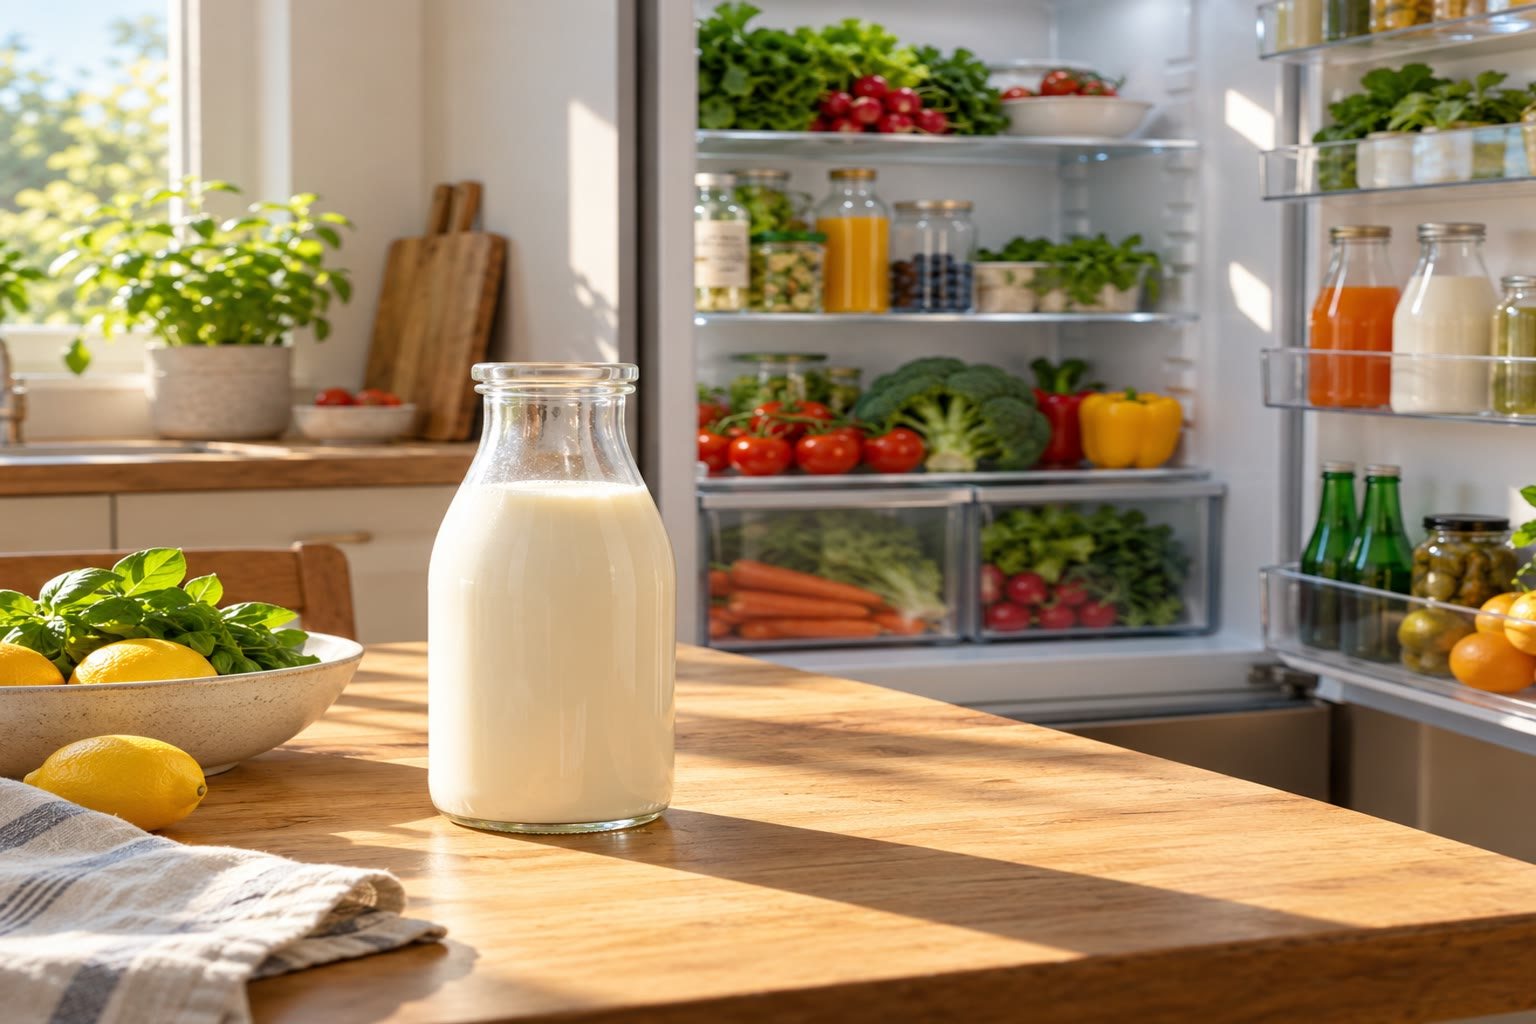
\includegraphics[width=0.55\linewidth]{images/book2/ai/b1-08-milk-kitchen.jpg}

{\small Sebotol susu yang dibiarkan di bawah sinar matahari di samping
lemari es yang terbuka. Reaksi-reaksi yang merusaknya berlangsung
beberapa kali lebih cepat pada suhu musim panas daripada dalam dingin.}
\end{omfigure}

\section{Laju sebuah reaksi}

\begin{definition}[Laju reaksi, laju pembentukan, dan laju penghilangan]\label{def:b1:rate-laws:rate}
Untuk reaksi $0 = \sum_i \nu_i\mathrm{A}_i$ yang berlangsung dalam reaktor
tertutup bervolume tetap $V$, \emph{laju reaksi}\index{laju reaksi}
adalah
\[
  v = \frac{1}{V}\frac{\dd\xi}{\dd t} = \frac{1}{\nu_i}\frac{\dd[\mathrm{A}_i]}{\dd t}
  \quad\text{(sembarang } i\text{)},
\]
dalam \unit{mol.L^{-1}.s^{-1}}. \emph{Laju pembentukan}\index{laju pembentukan}
sebuah produk adalah $\dd[\mathrm{A}_i]/\dd t$; \emph{laju
penghilangan}\index{laju penghilangan} sebuah pereaksi adalah
$-\dd[\mathrm{A}_i]/\dd t$.
\end{definition}

\begin{proposition}[Satu laju untuk semua spesies]\label{prop:b1:rate-laws:rate-relations}
\omterm{def:b1:rate-laws:rate}{Laju reaksi} tidak bergantung pada spesies yang dipilih untuk mengikutinya:
untuk $a\,\mathrm{A} + b\,\mathrm{B} \longrightarrow c\,\mathrm{C} + d\,\mathrm{D}$,
\[
  v = -\frac1a\frac{\dd[\ce{A}]}{\dd t} = -\frac1b\frac{\dd[\ce{B}]}{\dd t}
  = \frac1c\frac{\dd[\ce{C}]}{\dd t} = \frac1d\frac{\dd[\ce{D}]}{\dd t} .
\]
\end{proposition}

\begin{proof}
$[\mathrm{A}_i] = (n_{i,0} + \nu_i\xi)/V$ dengan $V$ tetap, sehingga
$\dd[\mathrm{A}_i]/\dd t = (\nu_i/V)\,\dd\xi/\dd t = \nu_i v$.
\end{proof}

\begin{example}[Penguraian dinitrogen pentoksida]\label{ex:b1:rate-laws:n2o5}
Untuk \ce{2N2O5 -> 4NO2 + O2}: $v = -\frac12\frac{\dd[\ce{N2O5}]}{\dd t} =
\frac14\frac{\dd[\ce{NO2}]}{\dd t} = \frac{\dd[\ce{O2}]}{\dd t}$. Nitrogen
dioksida muncul empat kali lebih cepat daripada dioksigen, dan dinitrogen
pentoksida hilang dua kali lebih cepat daripada munculnya dioksigen.
\end{example}

\section{Hukum laju dan orde}

\begin{definition}[Hukum laju, orde, tetapan laju]\label{def:b1:rate-laws:order}
\emph{Hukum laju}\index{hukum laju} menyatakan laju sebagai fungsi
konsentrasi. Sebuah reaksi \emph{mempunyai orde} jika hukum lajunya
berbentuk
\[
  v = k\,[\mathrm{A}]^{p}\,[\mathrm{B}]^{q} \cdots ;
\]
pangkat-pangkat $p$, $q$, \dots\ adalah \emph{orde parsial}\index{orde parsial}
terhadap A, B, \dots, jumlahnya adalah \emph{orde
total}\index{orde total}, dan $k$ adalah \emph{tetapan laju}\index{tetapan laju},
yang hanya bergantung pada suhu. Orde ditentukan melalui eksperimen;
orde tidak harus sama dengan koefisien stoikiometri, dan dapat berupa
pecahan atau nol.
\end{definition}

\begin{remark}[Satuan $k$]\label{rem:b1:rate-laws:units}
Karena $v$ dinyatakan dalam \unit{mol.L^{-1}.s^{-1}}, $k$ dinyatakan dalam
\unit{mol.L^{-1}.s^{-1}} untuk orde 0, \unit{s^{-1}} untuk orde 1,
\unit{L.mol^{-1}.s^{-1}} untuk orde 2, dan secara umum
$(\unit{mol/L})^{1-n}\,\unit{s^{-1}}$ untuk \omterm{def:b1:rate-laws:order}{orde total} $n$. Satuan $k$
menunjukkan \omterm{def:b1:rate-laws:order}{orde totalnya}.
\end{remark}

\begin{remark}[Reaksi tanpa orde]\label{rem:b1:rate-laws:no-order}
Tidak setiap reaksi mempunyai orde. Laju sebagian reaksi berupa pecahan
yang penyebutnya memuat konsentrasi, atau bergantung pada konsentrasi
sebuah produk. Hukum-hukum laju semacam itu dijelaskan oleh mekanisme
reaksinya (\cref{ch:b1:elementary-steps}). Sebuah reaksi juga dapat
mempunyai orde hanya pada awalnya: \omterm{def:b1:rate-laws:order}{hukum laju} awal.
\end{remark}

\section{Hukum laju terintegrasi dan waktu paruh}

\begin{definition}[Waktu paruh]\label{def:b1:rate-laws:half-life}
\emph{Waktu paruh}\index{waktu paruh} $t_{1/2}$ sebuah pereaksi adalah
waktu yang diperlukan untuk menghabiskan separuh jumlah awalnya.
\end{definition}

\begin{theorem}[Hukum laju terintegrasi]\label{thm:b1:rate-laws:integrated}
Untuk reaksi $a\mathrm{A} \rightarrow \text{produk}$ dengan laju $v = -\frac1a\frac{\dd[\ce{A}]}
{\dd t} = k[\ce{A}]^n$, dengan $[\ce{A}](0) = a_0$:
\begin{center}
\begin{tabular}{llll}
\hline
orde & hukum terintegrasi & grafik linear & \omterm{def:b1:rate-laws:half-life}{waktu paruh} \\
\hline
0 & $[\ce{A}] = a_0 - akt$ & $[\ce{A}]$ terhadap $t$ & $a_0/(2ak)$ \\
1 & $[\ce{A}] = a_0\,\eu^{-akt}$ & $\ln[\ce{A}]$ terhadap $t$ & $\ln2/(ak)$ \\
2 & $\dfrac{1}{[\ce{A}]} = \dfrac{1}{a_0} + akt$ & $1/[\ce{A}]$ terhadap $t$ & $1/(ak\,a_0)$ \\
\hline
\end{tabular}
\end{center}
\end{theorem}

\begin{proof}
Tuliskan $c = [\ce{A}]$, sehingga $\dd c/\dd t = -akc^n$.
\emph{Orde 0}: $\dd c/\dd t = -ak$, sehingga $c = a_0 - akt$ (berlaku
sampai $c = 0$). \emph{Orde 1}: $\dd c/\dd t = -akc$ adalah persamaan
diferensial linear orde satu yang penyelesaiannya $c = a_0\eu^{-akt}$.
\emph{Orde 2}: $\dd c/c^2 = -ak\,\dd t$; dengan mengintegralkan dari 0
sampai $t$, $-1/c + 1/a_0 = -akt$, sehingga $1/c = 1/a_0 + akt$. \omterm{def:b1:rate-laws:half-life}{Waktu
paruh}: substitusikan $c =
a_0/2$ ke dalam setiap hukum lalu selesaikan untuk $t$.
\end{proof}

\begin{proposition}[Uji waktu paruh]\label{prop:b1:rate-laws:half-life-test}
\omterm{def:b1:rate-laws:half-life}{Waktu paruh} tidak bergantung pada konsentrasi awal jika dan hanya jika
reaksinya berorde 1. \omterm{def:b1:rate-laws:half-life}{Waktu paruh} sebanding dengan $a_0$ untuk orde 0 dan
dengan $1/a_0$ untuk orde 2. Reaksi orde satu kehilangan separuh dari yang
tersisa pada setiap \omterm{def:b1:rate-laws:half-life}{waktu paruh} berikutnya: sesudah $m$ kali \omterm{def:b1:rate-laws:half-life}{waktu paruh},
tersisa bagian $2^{-m}$.
\end{proposition}

\begin{proof}
Untuk orde $n \ne 1$, pemisahan variabel menghasilkan $t_{1/2} = \dfrac{2^{n-1} -
1}{(n-1)\,ak\,a_0^{n-1}}$, yang bergantung pada $a_0$ kecuali jika $n = 1$;
untuk $n = 1$, $t_{1/2} = \ln2/(ak)$. Untuk orde 1, $c(t + t_{1/2}) = c(t)/2$
pada setiap $t$, karena $\eu^{-ak(t + t_{1/2})} = \eu^{-akt}/2$.
\end{proof}

\begin{omfigure}
\begin{tikzpicture}
\begin{axis}[name=p0,
  width=0.36\linewidth, height=4.6cm,
  xmin=0, xmax=60, ymin=0, ymax=1.05,
  axis x line=bottom, axis y line=left,
  xlabel={$t$ (min)}, title={orde 0: $[\ce{A}]$},
  title style={font=\small}, xtick={0,20,40,60},
  tick label style={font=\scriptsize}, label style={font=\small}]
\addplot[omDef, thick] table[x=t, y=A0] {figdata/out/bachelor-1-integrated-rate-laws.dat};
\end{axis}
\begin{axis}[at={(p0.east)}, anchor=west, xshift=0.9cm, name=p1,
  width=0.36\linewidth, height=4.6cm,
  xmin=0, xmax=60, ymin=-3.2, ymax=0.2,
  axis x line=bottom, axis y line=left,
  xlabel={$t$ (min)}, title={orde 1: $\ln[\ce{A}]$},
  title style={font=\small}, xtick={0,20,40,60},
  tick label style={font=\scriptsize}, label style={font=\small}]
\addplot[omProp, thick] table[x=t, y=lnA1] {figdata/out/bachelor-1-integrated-rate-laws.dat};
\end{axis}
\begin{axis}[at={(p1.east)}, anchor=west, xshift=0.9cm,
  width=0.36\linewidth, height=4.6cm,
  xmin=0, xmax=60, ymin=0, ymax=4.2,
  axis x line=bottom, axis y line=left,
  xlabel={$t$ (min)}, title={orde 2: $1/[\ce{A}]$},
  title style={font=\small}, xtick={0,20,40,60},
  tick label style={font=\scriptsize}, label style={font=\small}]
\addplot[omThm, thick] table[x=t, y=invA2] {figdata/out/bachelor-1-integrated-rate-laws.dat};
\end{axis}
\end{tikzpicture}

\begin{tikzpicture}
\begin{axis}[
  width=0.62\linewidth, height=5.0cm,
  xmin=0, xmax=60, ymin=0, ymax=1.05,
  axis x line=bottom, axis y line=left,
  xlabel={$t$ (min)}, ylabel={$[\ce{A}]$ (mol/L)}, xtick={0,10,20,30,40,50,60},
  tick label style={font=\small}, label style={font=\small},
  legend style={font=\small, draw=none, at={(0.98,0.98)}, anchor=north east}]
\addplot[omDef, thick] table[x=t, y=A0] {figdata/out/bachelor-1-integrated-rate-laws.dat};
\addplot[omProp, thick] table[x=t, y=A1] {figdata/out/bachelor-1-integrated-rate-laws.dat};
\addplot[omThm, thick] table[x=t, y=A2] {figdata/out/bachelor-1-integrated-rate-laws.dat};
\legend{orde 0, orde 1, orde 2}
\draw[dotted] (axis cs:0,0.5) -- (axis cs:20,0.5);
\end{axis}
\end{tikzpicture}

{\small Tiga reaksi dengan konsentrasi awal yang sama (\qty{1.00}{mol/L})
dan \omterm{def:b1:rate-laws:initial-rate}{laju awal} yang sama (\qty{0.050}{mol.L^{-1}.min^{-1}}). Atas: setiap
hukum terintegrasi menjadi garis lurus dalam koordinatnya sendiri.
Bawah: konsentrasinya; \omterm{def:b1:rate-laws:half-life}{waktu paruhnya} 10, 13.9, dan 20 menit.}
\end{omfigure}

\section{Menentukan hukum laju}

\begin{method}[Metode integral]\label{met:b1:rate-laws:integral}
Untuk menguji sebuah orde dengan data pengukuran $[\ce{A}](t)$: buatlah
grafik $[\ce{A}]$, $\ln[\ce{A}]$, dan $1/[\ce{A}]$ terhadap $t$; grafik
yang berupa garis lurus menunjukkan ordenya, dan kemiringannya
menghasilkan $k$ (kemiringan berturut-turut $-ak$, $-ak$, atau $+ak$).
\end{method}

\begin{method}[Metode waktu paruh]\label{met:b1:rate-laws:half-life}
Ukurlah \omterm{def:b1:rate-laws:half-life}{waktu paruh} untuk beberapa konsentrasi awal: tetap, orde 1;
sebanding dengan $a_0$, orde 0; sebanding dengan $1/a_0$, orde 2. Dalam
satu percobaan, bandingkan waktu untuk berubah dari $a_0$ ke $a_0/2$ dan
dari $a_0/2$ ke $a_0/4$: waktu yang sama berarti orde 1.
\end{method}

\begin{definition}[Laju awal]\label{def:b1:rate-laws:initial-rate}
\emph{Laju awal}\index{laju awal} $v_0$ adalah laju pada $t = 0$, yang
dibaca sebagai kemiringan garis singgung di titik asal kurva
$[\ce{A}](t)$, dibagi dengan koefisien stoikiometrinya. Pada saat itu
konsentrasi-konsentrasinya adalah konsentrasi awal yang diketahui dan
tidak ada produk yang mengganggu.
\end{definition}

\begin{method}[Metode laju awal]\label{met:b1:rate-laws:initial-rates}
Untuk $v_0 = k[\ce{A}]_0^p[\ce{B}]_0^q$: lakukan percobaan-percobaan yang
hanya mengubah $[\ce{A}]_0$; maka $\ln v_0 = \ln(k[\ce{B}]_0^q) + p\ln[\ce{A}]_0$,
dan kemiringan $\ln v_0$ terhadap $\ln[\ce{A}]_0$ adalah $p$. Dalam
praktik, menggandakan $[\ce{A}]_0$ mengalikan $v_0$ dengan $2^p$. Lakukan
hal yang sama untuk B.
\end{method}

\begin{definition}[Metode isolasi, orde semu]\label{def:b1:rate-laws:apparent-order}
Dalam \emph{metode isolasi}\index{metode isolasi}, semua pereaksi kecuali
satu dibuat sangat berlebih (sepuluh kali atau lebih). Konsentrasinya
praktis tetap, dan $v = k[\ce{A}]^p[\ce{B}]^q \approx k'[\ce{A}]^p$
dengan $k' = k[\ce{B}]_0^q$: reaksi itu berperilaku seakan-akan
mempunyai \emph{orde semu}\index{orde semu} $p$ dengan \omterm{def:b1:rate-laws:order}{tetapan laju} semu $k'$.
Hal ini disebut juga degenerasi orde.
\end{definition}

\begin{omfigure}
\begin{tikzpicture}
\begin{axis}[
  width=0.55\linewidth, height=4.8cm,
  xmin=0, xmax=40, ymin=0, ymax=1.05,
  axis x line=bottom, axis y line=left,
  xlabel={$t$ (min)}, ylabel={$[\ce{A}]$ (mol/L)},
  xtick={0,10,20,30,40},
  tick label style={font=\small}, label style={font=\small}, clip mode=individual]
\addplot[omProp, thick] table[x=t, y=A1] {figdata/out/bachelor-1-integrated-rate-laws.dat};
\draw[omThm, thick] (axis cs:0,1) -- (axis cs:20,0);
\node[omThm, anchor=west, font=\small] at (axis cs:2,0.12) {tangen di $t = 0$};
\end{axis}
\end{tikzpicture}

{\small Membaca \omterm{def:b1:rate-laws:initial-rate}{laju awal}: garis singgung di titik asal (merah) kurva orde
satu memotong sumbu waktu pada $t_0 = \qty{20}{min}$, sehingga $v_0 =
\qty{1.00}{mol/L}/\qty{20}{min} = \qty{0.050}{mol.L^{-1}.min^{-1}}$.}
\end{omfigure}

\begin{inthelab}[Mengikuti reaksi terhadap waktu]
Sebuah \omterm{def:b1:rate-laws:order}{hukum laju} disusun dari konsentrasi-konsentrasi yang diukur selama
reaksi berlangsung. Jika sebuah pereaksi atau produk berwarna,
spektrofotometer merekam absorbansnya, yang sebanding dengan
konsentrasinya (Beer--Lambert, \cref{ch:b1:structure-spectroscopy}); jika
ion-ion muncul atau hilang, konduktometer mengikuti konduktivitasnya;
jika terbentuk gas dalam bejana tertutup, manometer mengikuti tekanannya.
Jika tidak, sampel-sampel diambil pada waktu-waktu yang diketahui,
reaksinya dihentikan (dipadamkan) dengan pendinginan atau pengenceran,
dan setiap sampel dititrasi. Suhu bejana dijaga tetap dengan penangas
termostat, karena $k$ sangat bergantung padanya.
\end{inthelab}

\section{Suhu: hukum Arrhenius}

\begin{definition}[Energi aktivasi]\label{def:b1:rate-laws:activation-energy}
\emph{Energi aktivasi}\index{energi aktivasi} $E_a$ sebuah reaksi yang
\omterm{def:b1:rate-laws:order}{tetapan lajunya} $k(T)$ didefinisikan oleh
\[
  \frac{\dd \ln k}{\dd T} = \frac{E_a}{RT^2} ,
\]
dalam \unit{J/mol}. Jika $E_a$ tidak bergantung pada $T$, pengintegralan
menghasilkan $k = A\,\eu^{-E_a/RT}$, dengan tetapan $A$, yang satuannya
sama dengan satuan $k$, adalah \emph{faktor praeksponensial}\index{faktor praeksponensial}.
\end{definition}

\begin{theorem}[Hukum Arrhenius]\label{thm:b1:rate-laws:arrhenius}
Untuk sebagian besar reaksi, pada rentang suhu yang sedang, \omterm{def:b1:rate-laws:order}{tetapan laju}
mengikuti \emph{hukum Arrhenius}\index{hukum Arrhenius}
\[
  k(T) = A\,\eu^{-E_a/RT} ,
\]
dengan $A$ dan $E_a > 0$ tidak bergantung pada $T$: $\ln k$ adalah fungsi
linear $1/T$ dengan kemiringan $-E_a/R$.
\end{theorem}
\admitted

\begin{remark}[Makna $E_a$]\label{rem:b1:rate-laws:meaning}
Hukum ini empiris. Tafsirannya --- hanya tumbukan molekul yang membawa
energi sedikitnya berorde $E_a$ yang menghasilkan reaksi, dan bagian
tumbukan semacam itu berubah sebanding dengan $\eu^{-E_a/RT}$ --- dibuat
sketsanya bersama profil energi pada bab berikutnya dan dibuat
kuantitatif oleh teori-teori \omterm{def:b1:rate-laws:rate}{laju reaksi} dalam jilid Tahun 3.
\end{remark}

\begin{method}[Menentukan $E_a$]\label{met:b1:rate-laws:arrhenius-plot}
Dari \omterm{def:b1:rate-laws:order}{tetapan laju} pada beberapa suhu, buatlah grafik $\ln k$ terhadap
$1/T$ (dalam kelvin): kemiringannya $-E_a/R$, titik potongnya $\ln A$.
Dengan hanya dua suhu,
\[
  E_a = \frac{R\,\ln(k_2/k_1)}{1/T_1 - 1/T_2} .
\]
\end{method}

\begin{example}[Sebuah kaidah praktis]\label{ex:b1:rate-laws:doubling}
Untuk $E_a = \qty{53}{kJ/mol}$, naik dari 25 ke \qty{35}{\celsius}
mengalikan $k$ dengan $\exp\!\big(\frac{53000}{8.314}(\frac{1}{298.15} -
\frac{1}{308.15})\big) = 2.0$. Kaidah yang akrab ``sepuluh derajat lebih
panas, dua kali lebih cepat'' berlaku di sekitar suhu kamar untuk reaksi
berenergi aktivasi sekitar \qty{50}{kJ/mol}; untuk $E_a$ yang lebih besar
faktornya lebih besar.
\end{example}

\begin{omfigure}
\begin{tikzpicture}
\begin{axis}[
  width=0.6\linewidth, height=5.4cm,
  xmin=2.95, xmax=3.45, ymin=-9.0, ymax=-4.2, clip mode=individual,
  axis x line=bottom, axis y line=left,
  xlabel={$1000/T$ (\unit{K^{-1}})}, ylabel={$\ln k$ ($k$ dalam \unit{d^{-1}})},
  xtick={3.0,3.1,3.2,3.3,3.4}, ytick={-9,-8,-7,-6,-5},
  tick label style={font=\small}, label style={font=\small}]
\addplot[omDef, thick] table[x=invT_1e3, y=lnk] {figdata/out/bachelor-1-arrhenius-line.dat};
\addplot[only marks, mark=*, mark size=2.2pt, omThm] table[x=invT_1e3, y=lnk] {figdata/out/bachelor-1-arrhenius-points.dat};
\node[font=\small, anchor=south west] at (axis cs:3.002,-4.71) {\qty{60}{\celsius}};
\node[font=\small, anchor=south west] at (axis cs:3.095,-5.66) {\qty{50}{\celsius}};
\node[font=\small, anchor=south west] at (axis cs:3.193,-6.67) {\qty{40}{\celsius}};
\draw[dashed, black!50] (axis cs:3.354,-9.0) -- (axis cs:3.354,-8.31);
\addplot[only marks, mark=o, mark size=2.4pt, omDef] coordinates {(3.354,-8.310)};
\node[font=\small, anchor=east] at (axis cs:3.33,-8.40) {\qty{25}{\celsius}, ekstrapolasi};
\end{axis}
\end{tikzpicture}

{\small Grafik Arrhenius penguraian sebuah obat (soal akhir pekan): tiga
\omterm{def:b1:rate-laws:order}{tetapan laju} terukur (merah) terletak pada garis berkemiringan $-E_a/R$;
jika diekstrapolasikan ke \qty{25}{\celsius}, garis itu menghasilkan masa
simpan pada suhu kamar.}
\end{omfigure}

\begin{history}[Arrhenius, 1889]
Ahli kimia Swedia Svante Arrhenius, yang mempelajari inversi sukrosa oleh
asam pada tahun 1889, mengusulkan bahwa hanya sebagian kecil molekul,
yaitu yang berada dalam keadaan ``teraktifkan'', yang bereaksi, dan bahwa
bagian itu bertambah dengan suhu sebanding dengan $\eu^{-E/RT}$. Gagasan
itu, yang mula-mula diperdebatkan, menjadi fondasi kinetika kimia.
Arrhenius menerima Hadiah Nobel Kimia pada tahun 1903 untuk teorinya
tentang disosiasi elektrolitik.
\end{history}

\begin{omfigure}
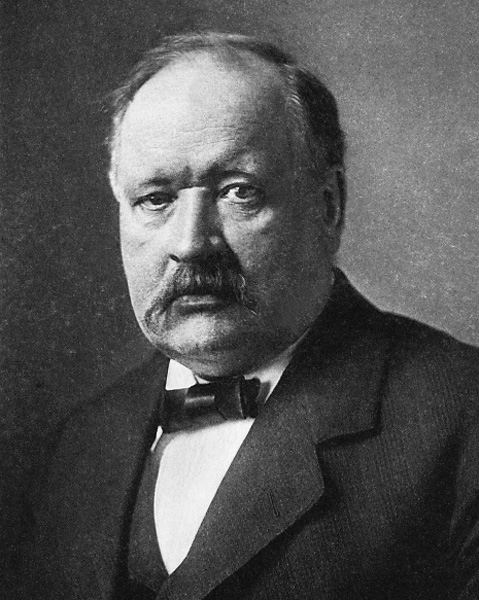
\includegraphics[width=0.22\linewidth]{images/book2/arrhenius.jpg}

{\small Svante Arrhenius (1859--1927), pada tahun 1909.}
\end{omfigure}

\section{Latihan}

\begin{exercise}[$\star$]\label{exo:b1:rate-laws:1}
Untuk \ce{2N2O5 -> 4NO2 + O2} pada volume tetap, nitrogen dioksida muncul
dengan laju $\qty{2.0e-4}{mol.L^{-1}.s^{-1}}$. Tentukan \omterm{def:b1:rate-laws:rate}{laju reaksi}, \omterm{def:b1:rate-laws:rate}{laju
pembentukan} dioksigen, dan \omterm{def:b1:rate-laws:rate}{laju penghilangan} \ce{N2O5}.
\end{exercise}

\begin{exercise}[$\star$]\label{exo:b1:rate-laws:2}
Tentukan satuan \omterm{def:b1:rate-laws:order}{tetapan laju} untuk \omterm{def:b1:rate-laws:order}{orde total} 0, 1, 2, dan 3, dengan
konsentrasi dalam \unit{mol/L} dan waktu dalam sekon.
\end{exercise}

\begin{exercise}[$\star$]\label{exo:b1:rate-laws:3}
Sebuah reaksi orde satu $\mathrm{A} \longrightarrow \mathrm{B}$ mempunyai $k = \qty{3.0e-3}{s^{-1}}$. Hitunglah
\omterm{def:b1:rate-laws:half-life}{waktu paruhnya} dan bagian \ce{A} yang tersisa sesudah \qty{10}{min}.
\end{exercise}

\begin{exercise}[$\star$]\label{exo:b1:rate-laws:4}
Jika konsentrasi awal sebuah pereaksi dibuat setengahnya, \omterm{def:b1:rate-laws:half-life}{waktu paruhnya}
menjadi dua kali lipat. Berapa ordenya? Bagaimana jika \omterm{def:b1:rate-laws:half-life}{waktu paruhnya}
menjadi setengahnya?
\end{exercise}

\begin{exercise}[$\star\star$]\label{exo:b1:rate-laws:5}
Konsentrasi sebuah pereaksi \ce{A} ($\mathrm{A} \longrightarrow \mathrm{P}$) diukur: pada $t
= 0$, 10, 20, 30, dan \qty{40}{min}, $[\ce{A}] = 0.100$, 0.0741, 0.0549,
0.0407, dan \qty{0.0301}{mol/L}. Tentukan orde dan \omterm{def:b1:rate-laws:order}{tetapan lajunya}.
\end{exercise}

\begin{exercise}[$\star\star$]\label{exo:b1:rate-laws:6}
Untuk $\mathrm{A} + \mathrm{B} \longrightarrow \mathrm{P}$, $v_0 = \qty{2.0e-6}{mol.L^{-1}.s^{-1}}$ untuk $[\ce{A}]_0
= [\ce{B}]_0 = \qty{0.010}{mol/L}$; \qty{8.0e-6}{} jika $[\ce{A}]_0$
digandakan; \qty{4.0e-6}{} jika $[\ce{B}]_0$ digandakan. Tentukan
orde-orde parsial, \omterm{def:b1:rate-laws:order}{hukum laju}, dan \omterm{def:b1:rate-laws:order}{tetapan lajunya}.
\end{exercise}

\begin{exercise}[$\star\star$]\label{exo:b1:rate-laws:7}
\omterm{def:b1:rate-laws:order}{Hukum laju} $\mathrm{A} + \mathrm{B} \longrightarrow \mathrm{P}$ adalah $v = k[\ce{A}][\ce{B}]$. Dengan
$[\ce{B}]_0 = \qty{0.50}{mol/L}$ dan $[\ce{A}]_0 = \qty{5.0e-3}{mol/L}$,
\ce{A} hilang menurut kinetika orde satu dengan tetapan semu
\qty{0.012}{s^{-1}}. Jelaskan, lalu hitunglah $k$.
\end{exercise}

\begin{exercise}[$\star\star$]\label{exo:b1:rate-laws:8}
Sebuah \omterm{def:b1:rate-laws:order}{tetapan laju} bernilai \qty{1.0e-3}{s^{-1}} pada \qty{300}{K} dan
\qty{5.0e-3}{s^{-1}} pada \qty{320}{K}. Hitunglah \omterm{def:b1:rate-laws:activation-energy}{energi aktivasi} dan
\omterm{def:b1:rate-laws:order}{tetapan laju} pada \qty{310}{K}.
\end{exercise}

\begin{exercise}[$\star\star$]\label{exo:b1:rate-laws:9}
Reaksi $2\,\mathrm{A} \longrightarrow \mathrm{P}$ mempunyai \omterm{def:b1:rate-laws:order}{hukum laju} $v = -\frac12\frac{\dd[\ce{A}]}
{\dd t} = k[\ce{A}]^2$ dengan $k = \qty{0.50}{L.mol^{-1}.s^{-1}}$. Mulai
dari $[\ce{A}]_0 = \qty{0.020}{mol/L}$, hitunglah \omterm{def:b1:rate-laws:half-life}{waktu paruh} dan
konsentrasi sesudah \qty{100}{s}.
\end{exercise}

\begin{exercise}[$\star\star\star$]\label{exo:b1:rate-laws:10}
Untuk reaksi orde satu, tunjukkan bahwa waktu yang diperlukan untuk
menghabiskan bagian $f$ pereaksi adalah $t_f = -\ln(1 - f)/(ak)$.
Bandingkan waktu untuk 50\,\%, 75\,\%, 90\,\%, dan 99.9\,\%, dalam
satuan \omterm{def:b1:rate-laws:half-life}{waktu paruh}.
\end{exercise}

\begin{exercise}[$\star\star\star$]\label{exo:b1:rate-laws:11}
Sebuah koyok kulit melepaskan obat dengan laju tetap \qty{0.40}{mg/h}
selama reservoirnya, yang semula \qty{10}{mg}, belum kosong. Tuliskan
hukum jumlah yang tersisa, tentukan ordenya, \omterm{def:b1:rate-laws:half-life}{waktu paruhnya}, dan waktu
sesudah koyok itu habis. Mengapa kinetika orde nol cocok untuk koyok
obat?
\end{exercise}

\begin{exercise}[$\star\star\star$]\label{exo:b1:rate-laws:12}
Tunjukkan bahwa kaidah ``sepuluh derajat lebih panas, dua kali lebih
cepat'' antara \qty{298.15}{K} dan \qty{308.15}{K} bersesuaian dengan
$E_a \approx
\qty{53}{kJ/mol}$. Faktor berapakah yang diberikan \omterm{def:b1:rate-laws:activation-energy}{energi aktivasi} yang
sama antara \qty{0}{\celsius} dan \qty{10}{\celsius}?
\end{exercise}

\section{Soal: Masa Simpan Sebuah Obat}

\begin{problem}[{Soal akhir pekan --- sebuah uji stabilitas dipercepat:
penguraian orde satu pada 60\,\textdegree C, tiga suhu, grafik Arrhenius,
dan masa simpan pada suhu kamar}]
\label{pb:b1:rate-laws:1}
Untuk meramalkan masa simpan $t_{90}$ sebuah tablet (waktu sesudah
10\,\% zat aktifnya terurai), sebuah laboratorium menyimpan sampel-sampel
pada suhu tinggi dan mengukur persentase zat aktif yang tersisa. Pada
\qty{60}{\celsius}:
\begin{center}
\begin{tabular}{lccccc}
\hline
waktu (hari) & 0 & 10 & 20 & 30 & 40 \\
zat aktif tersisa (\%) & 100.0 & 91.4 & 83.5 & 76.3 & 69.8 \\
\hline
\end{tabular}
\end{center}
Pada 40 dan \qty{50}{\celsius} \omterm{def:b1:rate-laws:order}{tetapan laju} yang diperoleh adalah
\qty{1.27e-3}{d^{-1}} dan \qty{3.48e-3}{d^{-1}}. Ambillah $R =
\qty{8.314}{J/(mol.K)}$ dan satu bulan $= \qty{30.4}{d}$.

\medskip
\noindent\textbf{Bagian I --- Orde pada 60\,\textdegree C.}
\begin{enumerate}
  \item Hitunglah pengurangan pada setiap selang 10 hari. Apakah reaksinya
        berorde 0?
  \item Hitunglah $\ln(\%\text{ tersisa})$ pada setiap waktu. Apa
        kesimpulannya?
  \item Turunkan \omterm{def:b1:rate-laws:order}{tetapan laju} $k_{60}$.
  \item Hitunglah \omterm{def:b1:rate-laws:half-life}{waktu paruh} pada \qty{60}{\celsius}.
  \item Berapa persen yang tersisa sesudah 60 hari pada \qty{60}{\celsius}?
  \item Hitunglah $t_{90}$ pada \qty{60}{\celsius}.
\end{enumerate}

\medskip
\noindent\textbf{Bagian II --- Masa simpan dan orde.}
\begin{enumerate}[resume]
  \item Tunjukkan bahwa untuk penguraian orde satu $t_{90} = \ln(10/9)/k$.
  \item Nyatakan $t_{90}$ sebagai bagian dari \omterm{def:b1:rate-laws:half-life}{waktu paruh}.
  \item Mengapa $t_{90}$ tidak bergantung pada dosis tablet?
  \item Mengapa laboratorium mengukur penguraian pada suhu tinggi dan
        bukan pada \qty{25}{\celsius}?
  \item Seandainya penguraian itu berorde 2 terhadap zat aktif, apakah
        tablet yang dua kali lebih kuat akan tahan lebih lama atau kurang
        lama? Jelaskan.
\end{enumerate}

\medskip
\noindent\textbf{Bagian III --- Grafik Arrhenius.}
\begin{enumerate}[resume]
  \item Tabelkan $1/T$ dan $\ln k$ untuk ketiga suhu itu.
  \item Hitunglah kemiringan garis yang melalui titik 40 dan
        \qty{60}{\celsius}.
  \item Turunkan \omterm{def:b1:rate-laws:activation-energy}{energi aktivasinya}.
  \item Periksalah bahwa titik \qty{50}{\celsius} terletak pada garis itu.
  \item Hitunglah \omterm{def:b1:rate-laws:activation-energy}{faktor praeksponensial} $A$.
  \item Dengan faktor berapakah laju bertambah antara 25 dan
        \qty{35}{\celsius}? Bandingkan dengan kaidah praktis itu.
\end{enumerate}

\medskip
\noindent\textbf{Bagian IV --- Suhu kamar.}
\begin{enumerate}[resume]
  \item Ekstrapolasikan \omterm{def:b1:rate-laws:order}{tetapan laju} ke \qty{30}{\celsius}.
  \item Hitunglah $t_{90}$ pada \qty{30}{\celsius}, dalam bulan.
  \item Sebuah kemasan tertinggal tiga hari di dalam mobil pada
        \qty{60}{\celsius}. Berapa bagian zat aktif yang hilang?
  \item Jelaskan petunjuk ``simpan di bawah \qty{25}{\celsius}''.
  \item Ekstrapolasikan \omterm{def:b1:rate-laws:order}{tetapan laju} ke \qty{25}{\celsius}.
  \item Hitunglah masa simpan $t_{90}$ pada \qty{25}{\celsius}, dalam hari
        dan dalam bulan.
\end{enumerate}
\end{problem}
